%%% VCU thesis/dissertation template file
\makeatletter
\let\my@xfloat\@xfloat
\makeatother

\documentclass[reqno]{vcuthesis}
\makeatletter
\def\@xfloat#1[#2]{
        \my@xfloat#1[#2]%
        \def\baselinestretch{1}%
        \@normalsize \normalsize
}
\makeatother
%%%%%%%%%%%%
% PACKAGES %
\usepackage{bm,amsmath,subfigure,graphicx,url,algorithm,algorithmicx,algpseudocode,booktabs}
\usepackage{tikz-cd,adjustbox,amsfonts,mathtools,tabularx,capt-of,longtable,comment,caption}
\usepackage[flushleft]{threeparttable}
\usepackage[top=1in,bottom=1in,right=1in,left=1in]{geometry}
\usepackage[backend=bibtex]{biblatex}
\usepackage[titletoc]{appendix}
\usepackage{pgfplots}
\pgfplotsset{compat=1.12}
\usepackage[linktocpage=true]{hyperref}
\usetikzlibrary{shapes.geometric,arrows,automata,positioning}
\usepackage{chngcntr}
\usepackage[final]{pdfpages}
\usepackage[explicit]{titlesec}

\newcommand{\iitem}{\item[-]}
\newcommand{\set}[1]{{\left\{#1\right\}}} 
\newcommand{\norm}[1]{{||#1||}} 
\newcommand{\st}{{\,|\,}} 
\newcommand{\reals}{{\mathbb{R}}}
\newcommand{\ints}{{\mathbb Z}}
\newcommand{\spa}[1]{\mathcal{#1}}
\newcommand\tab[1][1cm]{\hspace*{#1}}
\newcommand{\Rho}{\mathrm{P}}

%%%%%%%%%%%
\overfullrule=5pt
% BIBLIOGRAPHY %
\bibliography{../references}
\renewcommand{\type}{Dissertation}
\renewcommand{\thetable}{\arabic{table}}
\newcommand{\comments}[1]{}
%%%%%%%%%%%

% EQUATIONS %
\numberwithin{equation}{chapter}
%%%%%%%%%%%

% DOCUMENT  %
\begin{document}
\counterwithin{figure}{chapter}
\counterwithin{algorithm}{chapter}
\counterwithin{table}{chapter}

\pagenumbering{roman}

\makeatletter
\newcommand\pagenumberingnoreset[1]{\gdef\thepage{\csname @#1\endcsname\c@page}}
\makeatother

\tikzstyle{decision} = [diamond, draw, text centered, inner sep=3pt]
\tikzstyle{block} = [rectangle, draw, fill=gray!20,text width=5em, text centered, rounded corners, minimum height=4em]
\tikzstyle{arrow} = [thick,->,>=stealth]

%%%%%%%%%%%
\newcommand{\thesisordissertation}{Dissertation}
\newcommand{\thesistitle}{\uppercase\expandafter{} Novel Support Vector Machines for Diverse Learning Paradigms}
\newcommand{\authorsname}{Gabriella Angela Melki}
\newcommand{\thesismonth}{September}
\newcommand{\graduatingyear}{2018}
\newcommand{\degree}{Doctor of Philosophy}
\newcommand{\pastdegreeone}{Ph.D. Candidate}
\newcommand{\pastdegreetwo}{MSc. Computer Science, Virginia Commonwealth University, 2016} % 897 in .cls
\newcommand{\committeechair}{Alberto Cano}
\newcommand{\committeechairtwo}{Sebastian Ventura}
\newcommand{\major}{Computer Science}
\newcommand{\school}{Virginia Commonwealth University}
\newcommand{\chairposition}{Assistant Professor}
\newcommand{\chairpositiontwo}{Professor}
\newcommand{\majortwo}{Computer Science \& Numerical Analysis}
\newcommand{\schooltwo}{University of C\'{o}rdoba}

\vspace*{10em}
\begin{center}
\thispagestyle{empty}
\copyright Gabriella Angela Melki, September {\graduatingyear}\\
All Rights Reserved.
\end{center}
\vspace*{\fill}
\maketitlepage

\setlength{\headheight}{12pt}

\theabstract{\label{sec:abstractlabel}
This dissertation introduces novel support vector machines (SVM) for the traditional and non-traditional learning paradigms: \textit{Online Learning}, \textit{Multi-Target} Regression, \textit{Multiple-Instance} classification, and \textit{Data Stream} classification. 

Three multi-target support vector regression (SVR) models are first presented. The first involves building independent, single-target SVR models for each target. The second builds an ensemble of random chains using the first single-target method as a base model. The third calculates the targets' correlations and forms a maximum correlation chain, which is used to build a single chained SVR model, improving the model's prediction performance, while reducing computational complexity.

Under the multi-instance paradigm, a novel SVM multiple-instance formulation and an algorithm with a bag-representative selector, named MIRSVM, are presented. The contribution trains the SVM based on bag-level information and is able to identify instances that highly impact classification, i.e. bag-representatives, for both positive and negative bags, while finding the optimal class separation hyperplane. Unlike other multi-instance SVM methods, this approach eliminates possible class imbalance issues by allowing both positive and negative bags to have at most one representative, which constitute as the most contributing instances to the model.

\textbf{Add OLLAWV and DS Application}

Rigorous experimental studies and statistical analyses over various metrics and datasets were conducted in order to comprehensively compare the proposed solutions against modern, widely-used methods from both paradigms. The experimental study and analysis confirms that the proposals achieve better performances and more scalable solutions than the methods compared, making them competitive in their respected fields.
}\\

\pagenumberingnoreset{arabic}

\chapter{Introduction \label{chap:chapintro}}
In traditional classification and regression problems, learning algorithms attempt to correctly predict unknown samples by finding patterns between training samples and their outputs. Identifying these patterns is a non-trivial task due to many factors such as the high dimensionality of the data, as well as the dataset size. 

% first we can talk about volume of data
Over the past decade, dataset sizes have grown disproportionately to the speed of processors and memory capacity, limiting machine learning methods to computational time. Many real-world applications, such as human activity recognition, operations research, and video/signal processing, require algorithms that are scalable and accurate, while being able to provide insightful information in a timely fashion.

% then we introduce the notion of various types of data (mi and mt)
More recently, these traditional methods have been extended to accommodate various types of data paradigms. Examples include \textit{Multiple Target} (MT) learning  and \textit{Multiple Instance} (MI) learning. These emerging paradigms require algorithms to be robust and accommodate non-traditional data representations.

% introduce MT-Regression Problems
Multi-target learning is a challenging task that consists of creating predictive models for problems with multiple outputs. Specifically, MT learning is an approach to transfer learning that improves generalization by using domain information present in training data of multiple related targets as an inductive bias. This is done by learning in parallel, and what is learned for each target can be used to help other targets be learned better~\cite{Baxter1997,Caruana1997,thrun1996learning}. MT learning includes \textit{multi-target regression} (MTR), which addresses the prediction of continuous targets, \textit{multi-label classification}~\cite{Zhang20141819} which focuses on binary targets, and \textit{multi-dimensional classification} which describes the prediction of discrete targets~\cite{Borchani2015}. 

Multi-target prediction has the capacity to generate models representing a wide variety of real-world applications, ranging from natural language processing~\cite{Jeong2009} to bioinformatics~\cite{Lui2010}. A characteristic of the MT datasets used in these applications is that they are generated by a single system, indicating that the nature of the outputs captured has some structure. Even though modeling the multi-variate nature and possible complex relationships between the target variables is challenging, they are more accurately represented by a multi-target model~\cite{Caruana1997,Evgeniou2005}.

Several methods have been proposed for solving such multi-target tasks and can be categorized into two groups. The first being \textit{problem transformation} methods in which the multi-target problem is transformed into multiple single-target (ST) problems, each solved separately using standard classification and regression algorithms. The second being \textit{algorithm adaptation} methods which adapt existing traditional algorithms to predict all the target variables simultaneously~\cite{Borchani2015}. Using \textit{problem transformation} algorithms for a domain of \textit{t} target variables, \textit{t} predictive models must be constructed, each predicting a single-target variable. Prediction for an unseen sample would be obtained by running each of the \textit{t} single-target models and concatenating their results. Conversely, when using \textit{algorithm adaptation} algorithms for the same domain of \textit{t} target variables, a single model would need to be constructed which would output all \textit{t} predictions.

It is known that \textit{algorithm adaptation} methods outperform \textit{problem transformation} methods. The most valuable advantage of using multi-target techniques is that, not only are the relationships between the sample variables and the targets exploited, but the relationships between the targets amongst themselves are as well~\cite{Baxter1997,Caruana1997}. Single-target techniques, on the other hand, eliminate any possibility of learning from the possible relationships between the target variables because a single, independent model is trained for each target separately. Another advantage of MT techniques is model interpretability~\cite{BenDavic2003}. A single multi-target model is highly more interpretable than a series of single-target models. Not only is a single MT model more interpretable, but it could also be considerably more computationally efficient to train, rather than training multiple single-target models individually~\cite{evgeniou2004regularized}. 

Multi-instance learning (MIL) is a generalization of \textit{supervised learning} that has been recently been gaining interest because of its applicability to many real-world problems such as image classification and annotation \cite{Herman2008}, human action recognition \cite{Yi2016}, and drug activity prediction \cite{Dietterich1997}. The difference between MIL and traditional learning is the nature of the data. In the multi-instance setting, a sample is considered a \textit{bag} that contains multiple \textit{instances} and is associated with a single label. The individual instance labels within a bag are unknown and bag labels are assigned based on a multi-instance assumption, or hypothesis. Introduced by Dietterich et. al.~\cite{Dietterich1997}, the standard MI assumption states that a bag is labeled positive if and only if it contains at least one positive instance. Other hypotheses and frameworks have been proposed by Foulds and Frank~\cite{Foulds2010} to encompass a wider range of applications with MI data, but for the scope of this thesis, we will focus on the standard MI assumption.

One of the major complexities associated with MIL is the ambiguity of the relationship between a bag label and the instances within the bag. This stems from the standard MI assumption, where the underlying distribution among instances within positive bags is unknown. There have been different attempts to overcome this complexity, such as ``flattening" the MIL datasets, meaning instances contained in positive bags each adopt a positive label, allowing the use of classical supervised learning techniques~\cite{Ray2005}. This approach assumes that positive bags contain a significant number of positive instances, which may not be the case, causing the classifier to mislabel negative instances within the bag, decreasing the power of the MI model. To overcome this issue, a different MIL approach was proposed, where subsets of instances are selected from positive bags for classifier training~\cite{Maron1998}. One drawback of this type of method is that the resulting training datasets become imbalanced towards positive instances. Model performance further deteriorates when more instances are selected as subsets than needed~\cite{Carbonneau2016}. 

Our MTR and MIL proposals aim to deal with these drawbacks that exist in both paradigms using support vector machines. Support vector machines (SVM), proposed by Cortes and Vapnik~\cite{Cortes1995}, represent popular linear and non-linear (kernelized) learning algorithms based on the idea of a large-margin classifier. They have been shown to improve generalization performance for binary classification problems. SVMs are similar to other machine learning techniques, but literature shows that they usually outperform them in terms of scalability, computational efficiency, and robustness against outliers. They are known for creating sparse and non-linear classifiers, making them suitable for handling large datasets. A traditional approach for training SVMs is the \textit{Sequential Minimal Optimization} (SMO) algorithm~\cite{Platt1998}, a method for solving the L1-SVM's Quadratic Programming (QP) task. 

In this thesis, various approaches are devised for solving machine learning problems for various types of learning paradigms using traditional support vector machine solvers. Specifically, novel algorithms are proposed for solving multi-target regression (a subset of multi-target learning) and multi-instance classification problems. 

\section{Contributions of the Proposal \label{sec:introcontribute} }
% multi-target regression
The current leading MT models are based on ensembles of regressor chains, where random, differently ordered chains of the target variables are created and used to build separate regression models, using the previous target predictions in the chain. The challenges of building MT models stem from trying to capture and exploit possible correlations among the target variables during training, at the expense of increasing the computational complexity of model training. One of the contributions of this proposal aims to investigate the performance changes when building a regression model using two distinct \textit{algorithm adaptation} chaining methods versus building independent single-target models for each target variable using a novel framework. Specifically, this MTR contribution includes:
\begin{itemize}
\iitem Evaluating the performance of a Support Vector Regressor (SVR) as a multi-target to single-target \textit{problem transformation} method to determine whether it outperforms current popular ST algorithms. Its performance is analyzed as a base-line model for MT chaining methods due to the fact that ST methods do not account for any correlation among the target variables.
\newpage
\iitem Building an MT ensemble of randomly chained SVR models (SVRRC), an \textit{algorithm adaptation} approach, inspired by the chaining classification method, Ensemble of Random Chains Corrected (ERCC) {\cite{Spyromitros2014}}, to investigate the effects and advantages of exploiting correlations among target variables during model training, in the context of regression problems. The main issues to be investigated with this approach are the \textit{randomness} of the created chains because they might not capture of correlations between the targets, as well as the time taken to build all the regressors in the ensemble.

\iitem Proposing an MT \textit{algorithm adaptation} model of SVRs that builds a unique chain, capturing the maximum correlation among target outputs, named SVR Correlation Chains (SVRCC). The advantages of using this approach include exploiting the correlations among the targets which leads to an improvement in model prediction performance, and a reduction in computational complexity because a single SVR-chain model is trained, rather than building an ensemble of 10 base regressors.
\end{itemize}

To address the limitations presented by MIL algorithms, this thesis proposes a novel SVM formulation with a bag-representative selector, called Multiple-Instance Representative Support Vector Machine (MIRSVM). The algorithm does not assume any distribution of the instances and is not affected by the number of instances within a bag, making it applicable to a variety of contexts. The key contributions of this work include:
\begin{itemize}
\iitem Reformulating the traditional primal L$1$-SVM problem to optimize over bags, rather than instances, ensuring all the information contained within each bag is utilized during training, while defining bag representative selector criteria.

\iitem Deriving the dual multi-instance SVM problem, with the Karush-Kuhn-Tucker necessary and sufficient conditions for optimality. The dual is maximized with respect to the Lagrange multipliers and provides insightful information about the resulting sparse model. The dual formulation is kernelized with a Gaussian radial basis function, which calculates the distances between bag representatives.

\iitem Devising a unique bag-representative selection method that makes no presumptions about the underlying distributions of the instances within each bag, while maintaining the default MI assumption. This approach eliminates the issue of class imbalance caused by techniques such as flattening or subsetting positive instances from each bag. The key feature of MIRSVM is its ability to identify instances (support vectors) within positive and negative bags that highly impact the model.
\end{itemize}

\chapter{Background}
Support vector machines represent a popular set of learning techniques that have been introduced under Vapnik-Chervonenkis theory of \textit{structured risk minimization} (SRM)~\cite{boser1992training,Cortes1995,Kecman2001,Schoelkopf2002,Shalev2014}. SRM is an inductive principle for the purpose of model selection. It minimizes the expected probability of error, resulting in a generalized model, without making assumptions about the data distribution~\cite{Shalev2014,vapnik2015uniform}. This is the basis for developing the maximal margin classifier~\cite{vapnik2015uniform}. Based on the work of Aizerman et. al.~\cite{Aizerman67theoretical}, Boser et. al.~\cite{boser1992training} generalized the linear algorithm to the non-linear case. Then, Cortes and Vapnik~\cite{Cortes1995} proposed the soft margin SVM; a modification that not only allowed maximal margin classifiers to be applied to non-linearly separable data, but also introduced a regularization parameter to prevent overfitting and gauge generalizability. That same year, the algorithm was extended by Vapnik et. al.~\cite{vapnik2013nature} to the regression case.

This chapter presents a theoretical background of support vector machines. First, the SVM paradigm is discussed in the context of classification, introducing the concepts of the linear \textit{Hard Margin} classifier, and the nonlinear \textit{Soft Margin SVM}. Next, the concept of Support Vector Regression (SVR) is introduced. Afterwards, popular methods for solving the SVM problem are presented and their advantages and problems are discussed. 

\section{Support Vector Machine Classification}
Supervised learning is the process of determining a relationship $f(\bm x)$ by using a training dataset $\mathcal{S} = \{(\bm{x}_1,y_1),\ldots,(\bm{x}_i,y_i),\ldots,(\bm{x}_n,y_n)\}$, which contains $n$ inputs of $d$-dimensionality, $\bm x_i \in \reals^d$, and their class labels $y_i$. In the case of binary classification, $y_i \in \set{+1,-1}$, where $+1$ and $-1$ are the two class labels.

\begin{figure}[t!]
\centering
\begin{minipage}[b]{0.45\textwidth}
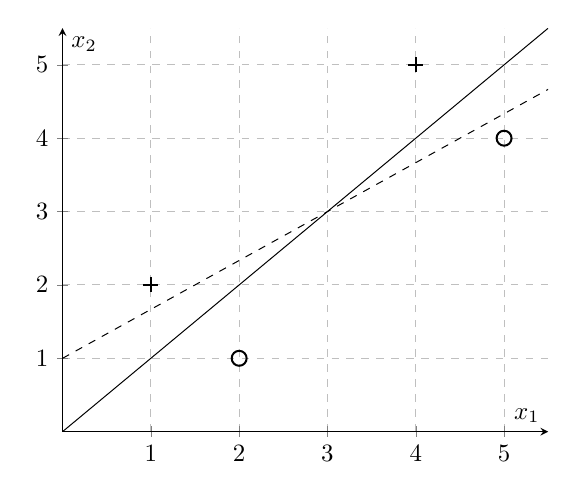
\begin{tikzpicture}[scale=0.9]
\begin{axis}[
    axis lines = center, xlabel = $x_1$, ylabel = $x_2$,
    xtick={0,1,2,3,4,5},ytick={0,1,2,3,4,5},
    ymajorgrids = true,xmajorgrids = true,grid style = dashed,]
%points defined +1
\addplot[only marks, thick, color=black, mark = +, mark size = 3pt]coordinates {(4,5)(1,2)};
%points defined -1
\addplot[only marks, thick, color = black, mark = o, mark size = 3pt]coordinates {(5,4)(2,1)};
%Below the black line is defined
\addplot [dashed,domain = 0:5.5, samples = 10, color = black,]{1/1.5 * x + 1};
%The gray line is defined
\addplot [domain = 0:5.5, samples = 10, color = black,]{x};
\end{axis}
\end{tikzpicture}
\caption{A 2-dimensional example of different possible separating hyperplanes that correctly classify all the toy data points.}
\label{fig:possiblesephyp}
\end{minipage}
\hfill
\begin{minipage}[b]{0.45\textwidth}
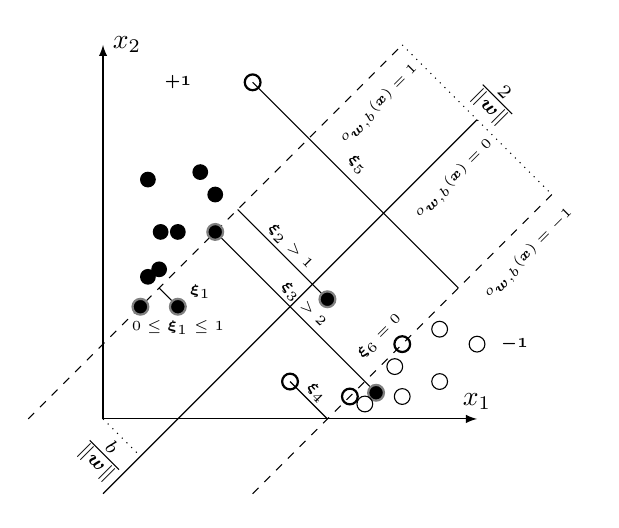
\begin{tikzpicture}[scale = 0.95]
  % Draw axes
  \draw [-latex] (0,0)--(0,5) node  [right]{$x_2$};
  \draw [-latex] (0,0)--(5,0) node  [above]{$x_1$};
  % draw line
  \draw (0,-1) -- (5,4); % y=x-1
  \draw[dashed] (-1,0) -- (4,5); % y=x+1
  \draw[dashed] (2,-1) -- (6,3); % y=x-3
  % \draw labels
  \draw (4.7,3.2) node[rotate=45,font=\tiny] {$o_{\bm w,b}(\bm{x}) = 0$};
  \draw (3.7,4.2) node[rotate=45,font=\tiny] {$o_{\bm w,b}(\bm{x}) = 1$};
  \draw (5.7,2.2) node[rotate=45,font=\tiny] {$o_{\bm w,b}(\bm{x}) = -1$};
  % draw distance
  \draw[dotted] (4,5) -- (6,3);
  \draw (5.25,4.25) node[rotate=-45] {$\frac{2}{\Vert \bm{w} \Vert}$};
  \draw[dotted] (0,0) -- (0.5,-0.5);
  \draw (0,-0.5) node[rotate=-45] {$\frac{b}{\Vert \bm{w} \Vert}$};
  \draw (1,1.5) -- (0.75,1.75);
  \draw (1.3,1.7) node [font=\tiny] {$\bm{\xi}_1$};
  \draw (1,1.225) node [font=\tiny] {$0 \leq \bm{\xi}_1 \leq 1$};
  \draw (3,1.6) -- (1.8,2.8);
  \draw (2.5,2.3) node [rotate=-45, font=\tiny] {$\bm{\xi}_2 > 1$};
  \draw (3.65,0.35) -- (1.5,2.5);
  \draw (2.675,1.525) node [rotate=-45, font=\tiny] {$\bm{\xi}_3 > 2$};
  \draw (2.5,0.5) -- (3,0);
  \draw (2.85,0.35) node [rotate=-45, font=\tiny] {$\bm{\xi}_4$};
  \draw (2,4.5) -- (4.75,1.75);
  \draw (3.4,3.4) node [rotate=-45, font=\tiny] {$\bm{\xi}_5$};
  \draw (5.5,1) node [font=\tiny] {$\bm{-1}$};
  \draw (1,4.5) node [font=\tiny] {$\bm{+1}$};
  \draw (3.7,1.1) node [rotate=45,font=\tiny] {$\bm{\xi}_6 = 0$};
  % draw negative dots
  \draw[thick, draw=gray, fill=black] 	(0.5,1.5) 	circle (3pt);
  \draw[thick, draw=gray, fill=black]   (1.5,2.5)   circle (3pt);
  \draw[thick, draw=gray, fill=black] 	(1,1.5)     circle (3pt);
  \draw[thick, draw=gray, fill=black] 	(3,1.6)     circle (3pt);
  \draw[thick, draw=gray, fill=black] 	(3.65,0.35)     circle (3pt);
  \fill[black] 	(1,2.5)     circle (3pt);
  \fill[black] 	(0.75,2)    circle (3pt);
  \fill[black] 	(0.6,1.9)   circle (3pt);
  \fill[black] 	(0.77, 2.5) circle (3pt);
  \fill[black] 	(1.5,3)     circle (3pt);
  \fill[black] 	(1.3,3.3)   circle (3pt);
  \fill[black] 	(0.6,3.2)   circle (3pt);
  % draw positive dots
  \draw[black,thick] (4,1)     circle (3pt); 
  \draw[black,thick] (3.3,.3)  circle (3pt); 
  \draw[black,thick] (2,4.5)  circle (3pt);
  \draw[black,thick] (2.5,0.5)  circle (3pt);
  \draw[black]     (4.5,1.2) circle (3pt); 
  \draw[black]     (4.5,.5)  circle (3pt); 
  \draw[black]     (3.9,.7)  circle (3pt); 
  \draw[black]     (5,1)     circle (3pt); 
  \draw[black]     (3.5,.2)  circle (3pt); 
  \draw[black]     (4,.3)    circle (3pt); 
\end{tikzpicture}
\caption{An illustration of the soft margin SVM solution on an example $2$-dimensional non-linearly separable dataset.}
\label{fig:nonlinsepdata}
\end{minipage}
\end{figure}

The goal of the soft margin SVM classifier is to find a classification function
\begin{equation}
\centering
f(\bm x) = \textsc{sign } o_{\bm w,b}(\bm x),
\label{eq:classificationfunction}
\end{equation}
where $o_{\bm w,b}(\bm x) = \bm{w}\cdot\bm{x}_i+b$ is a linear decision (output) function representing an affine mapping function $o: \reals^d \rightarrow \reals$ and is parameterized by $\bm w \in \reals^d$, the weight vector, and $b \in \reals$, the bias term. In addition, $\bm w$ and $b$ must satisfy the following,
\begin{equation}
y_i\left( \bm{w} \cdot \bm{x}_i + b\right) \geq 1 - \xi_i, \forall i \in \{1,\ldots,n\},
\label{eqn:softsvmconstraint}
\end{equation}
where $\bm \xi \in \reals^n$ are the non-negative slack variables that allow for some classification error to account for overlapping datasets. The minimal distance between points belonging to opposite classes and the hyperplane is defined as the \textit{margin} and has a width equal to $\frac{2}{||\bm{w}||}$, which is why the $\norm{\bm w}$ must be minimal in order to maximize the margin. 

In the example shown in Figure~\ref{fig:possiblesephyp}, if the training data points are slightly moved, the solid line (with the larger margin) will still correctly classify all the instances, whereas the dotted line (with a much smaller margin, comparatively) will not. This illustrates that the location of the hyperplane has a direct impact on the classifiers generalization capabilities. The hyperplane with the largest margin is called the \textit{optimal separating hyperplane}. Figure~\ref{fig:nonlinsepdata} shows the optimal separating hyperplane for overlapping training data points, where the filled data points are from the $+1$ class and the non-filled data points are from the $-1$ class. The training data points on the separating hyperplane (the circled data points), whose decision function value equals $+1$ or $-1$, are called the \textit{support vectors}. 

The soft margin SVM problem is defined as follows,
\begin{equation}
\label{eq:softsvm}
\begin{aligned}
\min\limits_{(\bm{w},b)} &{\,\,\,\,} \frac{1}{2}||\bm{w}||^2 + C\sum_{i=1}^n \xi_i \\
\text{s.t.} & {\,\,\,\,} y_i\left( \bm{w} \cdot \bm{x}_i + b\right) \geq 1 - \xi_i, {\,\,} \forall i \in \{1,\ldots,n\} \\
 & {\,\,\,\,} \xi_i \geq 0, {\,\,} \forall i \in \{1,\ldots,n\},
\end{aligned}
\end{equation}
where the penalty parameter $C \in \reals$ controls the trade-off between margin maximization and classification error minimization, penalizing large norms and errors. 

Equation~\ref{eq:softsvm} can be rewritten as a regularized loss minimization problem by representing the constraints as the Hinge loss, given by:
\begin{equation}
\centering
L(y_i,\, o_{(w,b)}(\bm{x}_i)) = \max \set{0, 1 - y_i o_{(w,b)}(\bm{x}_i)},
\end{equation}
which penalizes errors satisfying the following: $ y_i o_{(w,b)}(\bm{x}_i) < 1$ and is a crucial element that facilitates the SVM model's sparseness. The soft margin SVM represented as a regularized loss minimization problem becomes:
\begin{equation}
\label{eqn:reghingeloss}
\min\limits_{\bm (\bm{w},b) \in \mathcal{H}_o \times \reals} R {\,\,} = {\,\,} \frac{1}{2}||\bm{w}||^2 + C\sum_{i=1}^n L(y_i,\, o_{(w,b)}(\bm{x}_i)),
\end{equation}
where $\mathcal{H}_o$ is a general Hilbert space. To handle cases when the data are non-linearly separable, while enhancing the classifier's generalization capabilities, a kernel function can be used~\cite{Aizerman67theoretical}, as shown in Equation~\ref{eq:kerneltrick}:
\begin{equation}
\spa{K}\left(\bm{x}_i,\bm{x}_j\right) = \langle \phi\left(\bm{x}_i\right),\,\phi\left(\bm{x}_j\right)\rangle,
\label{eq:kerneltrick}
\end{equation}
where $\phi(\cdot)$ represents a mapping function from the original feature space to a higher dimensional space. The advantage of utilizing kernels is being able to calculate the inner product in the input space rather than in the very high feature dimensional space (including the infinite dimensional ones). The SVM model output, $o$ shown in Equation~\ref{eq:output}, for a given input vector $\bm{x}$ is defined by the kernel as given below:
\begin{equation}
o(\bm x) = \sum_{i = 1}^n \alpha_i \mathcal{K}(\bm x, \bm{x}_i) + b,
\label{eq:output}
\end{equation}
where $\alpha_i \in \reals$ are the coefficients, or weights, of the expansion in feature space, and $b \in \reals$ is the so-called bias term. Note that if a positive definite kernel is used, there is no need for a bias term $b$, but $b$ can nevertheless be used. The two terms, $\bm \alpha$ and $b$, parametrize the SVM model. A model is called \textit{dense} if the absolute value of all its weights are greater than $0$, while a \textit{sparse} model would be one that contains some $\alpha_i = 0$. The level of sparseness may vary, but the sparser the model, the more scalable the applications.

\section{Support Vector Regression}
The support vector machine was applied to the regression case~\cite{Drucker1997,vapnik1997support}, maintaining all the maximal margin algorithmic features. Unlike pattern recognition problems where the desired outputs $y_i$ are discrete, for the regression case they are continuous, real-valued, function outputs. Given training dataset $\mathcal{S} = \set{(\bm x_1,y_1), \ldots, (\bm x_n,y_n) \in \reals^d \times \reals}$, where $y_i \in \reals$ is the continuous output of input $\bm x_i \in \reals^d$, the goal is to learn a function $f(\bm x)$ with at most $\epsilon$ deviation from the true targets $y_i$ for all the training data, while being as flat as possible. This was introduced by Vapnik's linear loss function with $\epsilon$-insensitivity zone, illustrated in Figure~\ref{fig:epsloss} and given by:
\begin{equation}
\label{eq:epsloss}
\centering
|y_i - o_{(w,b)}(\bm{x_i})|_\epsilon = \begin{cases} 
															0 & if |y_i - o_{(w,b)}(\bm{x_i})| \leq \epsilon \\
															|y_i - o_{(w,b)}(\bm{x_i})| - \epsilon & \text{otherwise}.
														\end{cases}
\end{equation}
The loss is equal to 0 if the difference between the predicted and true output values is less than $\epsilon$. Vapnik's $\epsilon$-insensitivity function, shown in Equation~\ref{eq:epsloss}, defines an $\epsilon$-tube, illustrated in Figure~\ref{fig:regressionsvm}. If the predicted value is within the tube, no loss is incurred~\cite{Kecman2001}. Estimating a linear regression hyperplane is achieved by minimizing:
\begin{equation}
\label{eq:regsvmemp}
\min\limits_{(\bm{w},b) \in \mathcal{H}_o \times \reals} R {\,\,} = {\,\,} \frac{1}{2}||\bm{w}||^2 + C\sum_{i=1}^n (|y_i - o_{(w,b)}(\bm{x_i})|_\epsilon).
\end{equation}
Equation~\ref{eq:regsvmemp} is equivalent to the following, where non-negative slack variables are introduced:
\begin{equation}
\label{eq:softsvropt}
\begin{aligned}
\min\limits_{(\bm{w},b,\bm \xi,\bm \xi^*)} & {\,\,\,\,} \frac{1}{2}||\bm{w}||^2 + C\sum_{i=1}^n{\left(\xi_i + \xi^*_i \right)} \\
\text{s.t.} & {\,\,\,\,} y_i - \bm{w} \cdot \bm{x}_i  - b \leq \xi_i + \epsilon, {\,\,} \forall i = \set{1,\ldots,n}\\
				 & {\,\,\,\,} \bm{w} \cdot \bm{x}_i + b - y_i \leq \xi_i^* + \epsilon, {\,\,} \forall i = \set{1,\ldots,n} \\
				 & {\,\,\,\,} \xi_i, \xi^*_i \geq 0, {\,\,} \forall i = \set{1,\ldots,n}.
\end{aligned}
\end{equation}
Note that the constant $C$ influences the trade-off between approximation error and the model generalizability, similar to the classification setting. 
\begin{figure}[t!]
\centering
\begin{minipage}[b]{0.45\textwidth}
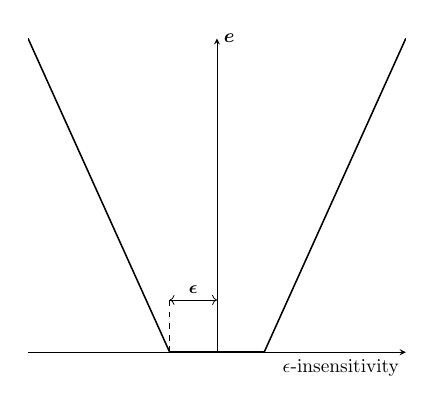
\begin{tikzpicture}[scale=0.7]
\begin{axis}[
	ticks=none,
    axis lines = center, 
    xlabel = $\epsilon\text{-insensitivity}$, 
    xlabel style={below left},
    ylabel = $\bm e$,
    ylabel style={ right}]
% negative epsilon intensity
\addplot [
	thick,
    domain=-4:-1, 
    samples=2, 
    color=black,
]
{- x - 1};
% 0 epsilon intensity
\addplot [
	very thick,
    color=black,
]
coordinates {(-1, 0) (1, 0)};
% positive epsilon intensity
\addplot [
	thick,
    domain=1:4, 
    samples=2, 
    color=black,
]
{ x - 1};
% vertical line indicating where epsilon begines
\addplot[
	color=black,
	style=dashed,
]
coordinates {(-1, 0) (-1, 0.5)};
% epsilon node
\draw[<->] (-1, 0.5) -- (0, 0.5);
\draw (-0.5,0.6) node[font=\small] {$\bm \epsilon$};
\end{axis}
\end{tikzpicture}
\caption{Vapnik's $\epsilon$-insensitivity loss function.}
\label{fig:epsloss}
\end{minipage}
\hfill
\begin{minipage}[b]{0.45\textwidth}
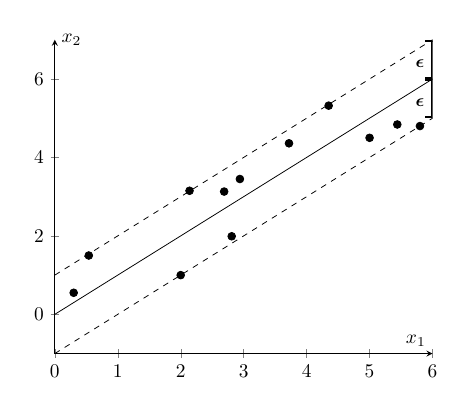
\begin{tikzpicture}[scale = 0.7]
\begin{axis}[
	%ticks = none, 
	axis lines = left, 
	xlabel = $x_1$, 
	xlabel style={at={(1,0)}, above left},
	ylabel = $x_2$,
	ylabel style={at={(0,1)}, right,rotate=-90}
    ]
% main function x
\addplot [
    domain=0:6, 
    samples=2, 
    color=black,
]
{x};
% margin function x + eps
\addplot [
	dashed,
    domain=0:6, 
    samples=2, 
    color=black,
]
{ x+1};
% margin function x - eps
\addplot [
	dashed,
    domain=0:6, 
    samples=2, 
    color=black,
]
{ x - 1};
% epsilon margin
\draw[|-|,very thick] (6,7) -- (6,6);
\draw[|-|,very thick] (6,6) -- (6,5);
\draw (5.8,6.4) node[font=\small] {$\bm \epsilon$};
\draw (5.8,5.4) node[font=\small] {$\bm \epsilon$};
\addplot[color=black,only marks, mark size=2] coordinates {(0.54,1.5) (2,1) (2.14,3.15) (2.94,3.45) (5.8,4.8) (0.30,0.55) (2.69,3.13) (2.81,1.99) (3.72,4.36) (4.35,5.32) (5.44,4.84) (5,4.5) };
\end{axis}
\end{tikzpicture}
\caption{Support vector regression example solution.}
\label{fig:regressionsvm}
\end{minipage}
\end{figure}
The optimization function given in~\ref{eq:softsvropt} can be solved more easily in its dual formulation and is key to extending the SVR to learn from non-linear functions~\cite{Schoelkopf2002}. It is as follows:
\begin{equation}
\label{eq:dualSVR}
\centering
\begin{aligned}
\max\limits_{(\bm \alpha, \bm \alpha^*)} & {\,\,\,\,} -\frac{1}{2} \sum_{i,j = 1}^n (\alpha_i - \alpha^*_i)(\alpha_j - \alpha^*_j)\mathcal{K}(\bm x_i, \bm x_j)  - \epsilon \sum_{i=1}^n (\alpha_i + \alpha^*_i) + \sum_{i=1}^n y_i (\alpha_i - \alpha^*_i) \\
 \text{s.t.} & {\,\,\,\,} \sum_{i=1}^n (\alpha_i - \alpha^*_i) = 0,\, \alpha_i, \alpha^*_i \in [0, C],\, \forall i = \set{1,\,\ldots,n},
 \end{aligned}
\end{equation}
where $\bm \alpha$ and $\bm \alpha^*$ correspond to the SVR dual variables.  

\section{Methods for Solving the SVM Problem}
Although support vector machines represent a major development in machine learning algorithms, in the case of large-scale problems (hundreds of thousands to several millions of samples), the design of SVM training algorithms still has room for improvement. So far, there have been various approaches for tackling large-scale SVM classification problems.

Interior Point (IP) methods (e.g.~\cite{Boyd2004}) pose the SVM learning problem as a quadratic optimization problem subject to linear constraints, which are then replaced with a barrier function. The resulting problem can then optimized using Newton or Quasi-Newton methods. However, IP methods typically require a run time of $O(n^3)$. Moreover, the memory requirements of IP methods are $O(n^2)$ rendering the use of IP methods impractical when the training set consists of a large number of samples. 

The first attempts of overcoming the quadratic memory requirement of IP methods and speeding up their training time were aimed at decomposing the underlying SVMs quadratic programming problem. First, Boser et al.~\cite{boser1992training} implemented Vapnik's \textit{chunking} method. \textit{Sequential Minimal Optimization} (SMO) by Platt~\cite{Platt1998}, its improvement by Keerthie et al.~\cite{keerthi2001improvements}, and SVM-Light~\cite{Joachims1999} are alternative approaches to \textit{decomposing} the QP problem. SMO, implemented in the popular, widely used software package LIBSVM~\cite{CC01a}, is an iterative procedure that divides the SVM dual problem into a series of sub-problems, which are solved analytically by finding the optimal $\bm \alpha$ values that satisfy the Karush-Kuhn-Tucker conditions~\cite{Boyd2004}. Although SMO is guaranteed to converge, heuristics are used to choose $\bm \alpha$ values in order to accelerate the convergence rate. This is a critical step because the convergence speed of the SMO algorithm is highly dependent on the dataset size and SVM hyperparameters~\cite{Schoelkopf2002}. 

Most existing approaches, including the methods described above, focus on solving the dual of Equation~\ref{eq:softsvm}, especially when used in conjunction with non-linear kernels. However, when using non-linear kernels, the Representer theorem~\cite{scholkopf2001generalized} enables the re-parameterization of the weight vector $\bm w$ to $\bm w = \sum_{i=1}^n \alpha_i y_i x_i$, and the primal SVM problem can then be cast as an unconstrained optimization problem with variables $\bm \alpha \in \reals^n$. Chapelle~\cite{Chapelle2007} investigated solving the primal objective with smooth loss functions instead of the hinge loss and suggested using methods such as the conjugate gradient descent and Newton's method.

Some advancements in handling large scale problems are based on a geometric interpretation of SVM problem. Some of these geometric SVMs include approaches that use convex hulls~\cite{bennett2000duality} and minimum enclosing balls such as \textit{Core Vector Machines} (CVM)~\cite{tsang2005core}. Tsang et al.~\cite{tsang2007simpler} then improved the scalability of CVMs by introducing \textit{Ball Vector Machines} (BVM) which do not require a QP solver. Other geometric approaches include the novel algorithms introduced by Strack~\cite{strack2013geometric}, known as the \textit{Sphere Support Vector Machine} (SphereSVM) and \textit{Minimal Norm Support Vector Machine} (MNSVM), which utilize the connection between minimal enclosing balls and convex hull problems, while demonstrating a high capability for learning from large datasets. 

The \textit{Non-Negative Iterative Single Data Algorithm} (NNISDA)~\cite{zigic2016} is an efficient approach for solving the SVM problem, shown to be faster than SMO and equal in terms of accuracy~\cite{Kecman2014}. NNISDA is an iterative algorithm that finds a solution to the L2-SVM using coordinate descent, inspired by \textit{Iterative Single Data Algorithm} (ISDA)~\cite{Huang2006} which was originally introduced by Kecman et al.~\cite{Kecman2005}.

Recently, several authors have proposed the use of a standard stochastic (or online) gradient descent (SGD) approach for SVMs to optimize large-scale learning problems~\cite{herbrich2016learning,kivinen2002large,Schoelkopf2002,Shalev2014,shalev2011pegasos}. Kivinen et al.\cite{kivinen2004online} and Bousquet and Bottou~\cite{bousquet2008tradeoffs} showed that stochastic algorithms can be both the fastest, and have the best generalization performances. Shalev-Shwartz and Ben-David~\cite{Shalev2014} have also demonstrated that the basic SGD algorithm is very effective when data are sparse, taking less than linear $[O(d)]$ time and space per iteration to optimize a system with $d$ parameters. It can greatly surpass the performance of more sophisticated batch methods on large data sets. The previously mentioned approaches are extended variants of a classic kernel perceptron algorithm~\cite{collobert2004links}. 

Notable representatives of this method of learning include the \textit{Na{\"i}ve Online R Minimization Algorithm} (NORMA) by Kivinen et al.~\cite{kivinen2004online} and the \textit{Primal Estimated Sub-Gradient SOlver for SVM} (PEGASOS) by Shalev-Shwartz et al.~\cite{shalev2011pegasos}. NORMA is an online kernel based algorithm designed to utilize SGD for solving the SVM problem, exploiting the kernel trick in an online setting. It can be regarded as a generalization of the kernel perceptron algorithm with regularization~\cite{kivinen2004online}. PEGASOS solves the primal SVM problem using stochastic sub-gradient descent, implementing both linear and non-linear kernels, and showed that the algorithm does not directly depend on the size of the data, making it suitable for large-scale learning problems. 

A more recent approach, named \textit{OnLine Learning Algorithm} (OLLA)~\cite{kecman2016fast} is a unification, simplification, and expansion of the somewhat similar approaches presented in
~\cite{herbrich2016learning,kivinen2002large,Schoelkopf2002,Shalev2014,shalev2011pegasos} and~\cite{kecman2016ieee,Melki2016,melki2016fast}. This algorithm is unique because it is not only designed to optimize the SVM cost function, but also the cost functions of several other popular nonlinear (kernel) classifiers using SGD in the primal domain. Collobert and Bengio~\cite{collobert2004links} provided justification for not using regularization, and thus OLLA was designed to handle cost functions with and without the regularization term. Comparisons of performances of OLLA with the popular SMO algorithm highlighted the merits of OLLA in terms of speed, as well as accuracy, when the number of samples was increased, making it suitable for large-scale learning. Comparisons using various different classifiers against SMO were also shown~\cite{kecman2016fast}, but for the scope of this proposal the L1-SVM was mentioned.

Although the SGD approaches mentioned above have many merits when it comes to solving large-scale machine learning problems, stochastic procedures also have their disadvantages. One of them stems from the lack of meaningful stopping criteria. The only specified stopping criteria is a user defined input for the number of iterations, which gives rise to the question of what it should be set to. Another disadvantage of kernelized online algorithms is that the training time for each update increases superlinearly with the number of samples. 

\section{Why SVMs: Form vs. Norm}

\end{document}